\chapter{Experimental Apparatus}
\label{chap:experiment}

What machines must we build to examine the smallest pieces of the universe? The famous equation 
$E = m$ provides that to create massive particles, we need to provide enough energy. In order to give 
kinematic phase space to the types of processes that are examined in this thesis (and many others besides),
a system must be created in which there is enough energy to (at bare minimum), overcome kinematic thresholds:
if you want to search for $HH$ decays, you should have at least \SI{250}{\GeV} ($= 2\times m_{H}$) to work with.
It is not enough to simply induce such processes, however. These processes need to be captured in some way, emitted 
energy and particles must be characterized and identified, and in the end all of this information must be put into a 
useful and useable form such that selections can be made, statistics can be run, and a meaningful statement 
can be made about the universe. In this chapter, we describe the machines behind the physics, namely the Large 
Hadron Collider and the ATLAS experiment.

\section{The Large Hadron Collider}
The Large Hadron Collider is a particle accelerator near Geneva, Switzerland, 
operating at a center of mass energy $\sqrt{s} = \SI{13}{\TeV}$. In broad scope, it is a 
ring with a 27 kilometer circumference. Hadrons (usually protons or heavy ions) move in two 
counter-circulating beams, which are made to collide at four collision points at various 
points on the ring. These four collision points correspond to the four detectors placed 
around the ring: two ``general purpose'' experiments: ATLAS and CMS; LHCb, focused primarily 
on flavor physics; and ALICE, focused primarily on heavy ions.

For proton-proton collisions, the focus of this thesis, the acceleration chain proceeds as follows:
first, and electric field strips hydrogen of its electrons, creating protons. A linear accelerator,
LINAC 2, accelerates protons to \SI{50}{\MeV}. The resulting beam is injected into the Proton 
Synchrotron Booster (PSB), which pushes the protons to \SI{1.4}{\GeV}, and then the Proton Synchrotron,
which brings the beam to \SI{25}{\GeV}.

Protons are then transferred to the Super Proton Synchrotron (SPS), which ramps up the energy to 
\SI{450}{\GeV}. Finally, the protons enter the LHC itself, bringing the beam up to \SI{6.5}{\TeV}. \todo{cite: https://home.cern/science/accelerators/accelerator-complex}

While there is, of course, much that goes into the Large Hadron Collider development and operation, perhaps
two of the most fundamental ideas are (1) how are the beams directed and manipulated and (2) what do we 
mean when we say ``protons are accelerated''. These questions both are directly answered by pieces of hardware,
namely (1) magnets and (2) radiofrequency (RF) cavities.

One of fundamental components of the LHC is a large set of superconducting magnets \todo{material?}. These 
are cooled by liquid helium to achieve superconducting temperatures, and there are several types with very 
specific purposes. The obvious first question with a circular accelerator is how to keep the particle beam 
moving around in that circle. This job is done via a set of dipole magnets placed around the \emph{beam pipes}: the 
tubes containing the beam. These are designed such that the magnetic field in the center of the beam pipe runs 
perpendicular to the velocity of the charged particles, providing the necessary centripetal force for 
the synchrotron motion.

A proton beam is not made of a single proton, however, but of many protons, grouped into a series of \emph{bunches}.
As all of these are positively charged, if unchecked, these bunches would become diffuse and break apart. What we 
want is a stable beam with tightly clustered protons to maximize the chance of a high energy collision.
Such clustering is done via a series of quadropole magnets, with field distributed as in 
\todo{grab image from General Exam}. Alternating sets of quadropoles provide the necessary forces for a tight, 
stable beam. While these are the two major components of the LHC magnet system, it is not the full story -- higher order 
magnets are used to correct for small imperfections in the beam \todo{expand}.

Magnetic fields do no work, however, so the magnet system is unable to do the job of the actual acceleration. This is 
accomplished via a set of radiofrequency (RF) cavities. Within these cavities, an electric field is made to 
oscillate (switch direction) at a precise rate. These rates interact with the beam via in RF \emph{buckets}, with 
bunches corresponding to groups of protons that fill a given bucket. The timing is such that protons will always 
experience an accelerating voltage, corresponding to the \SI{25}{\ns} bunch spacing used at the LHC.

A nice property of this bucket/bunch configuration is that there is some self-correction -- there is 
some finite spread in the grouping of particles. If a particle arrives too early, it will experience some 
decelerating voltage; if too late, it will experience a higher accelerating voltage.


\section{The ATLAS Experiment}
\label{sec:ATLAS}

\begin{figure}[ht]
\centering
\subfloat{
		  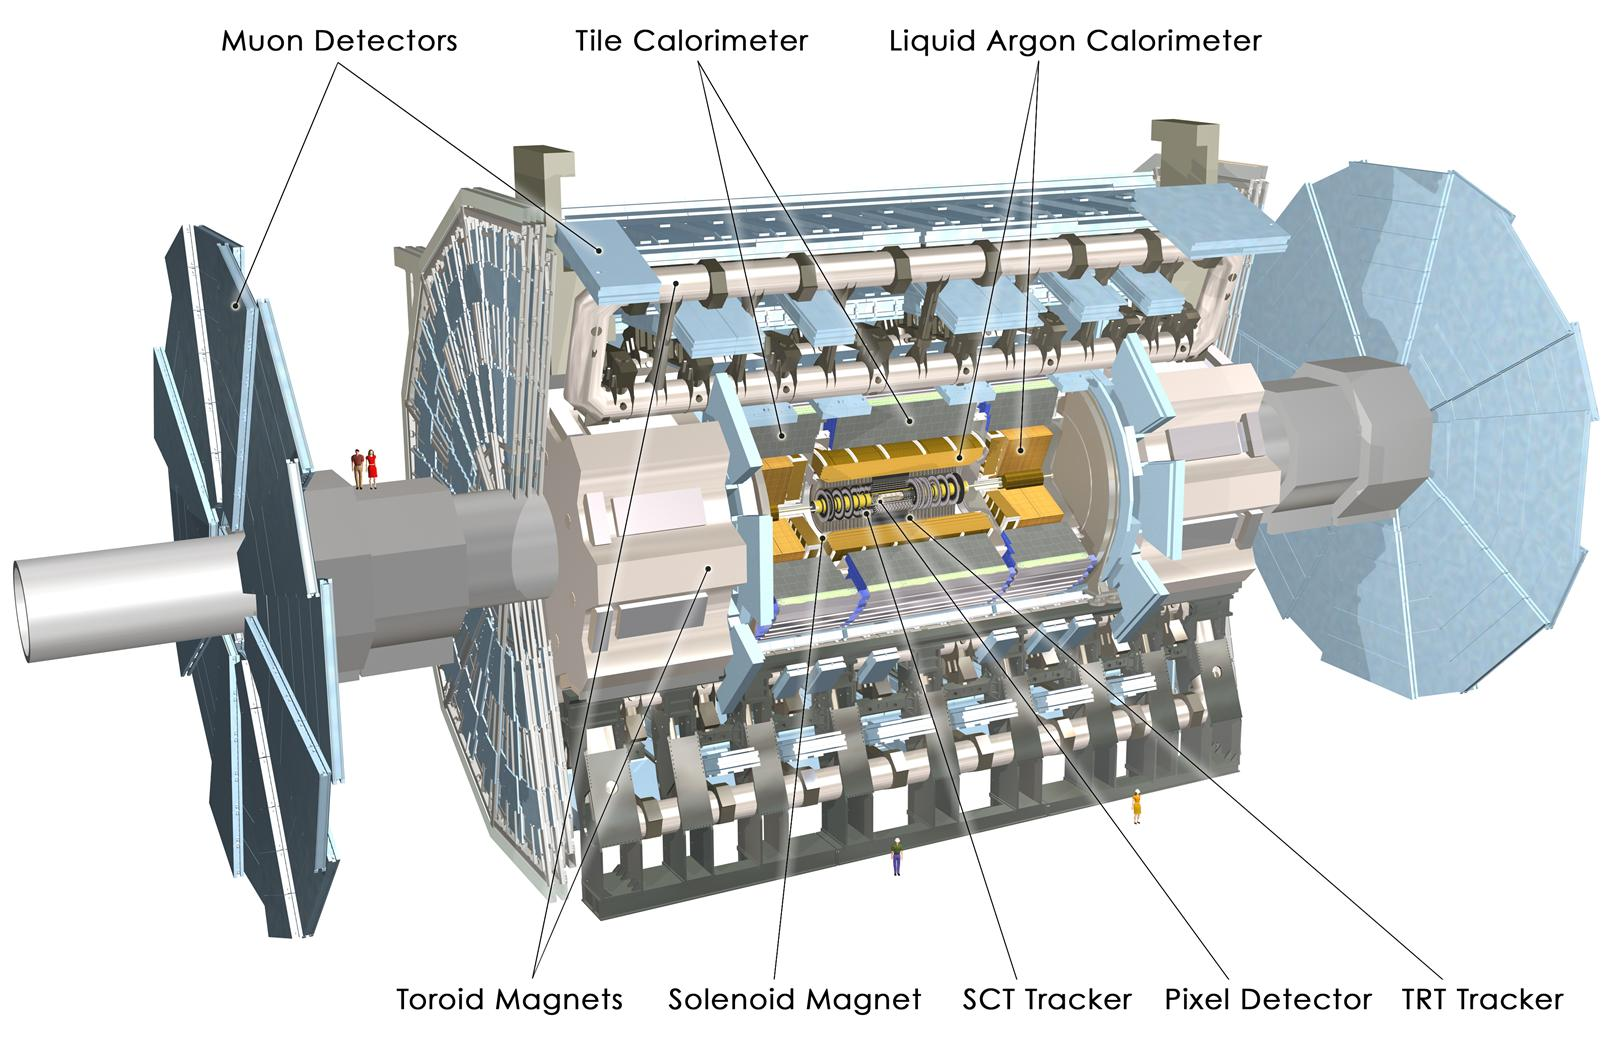
\includegraphics[width=0.8\textwidth]{figures/ATLAS-det.jpeg}
		 }
\caption{Diagram of the ATLAS detector \cite{DetectorImage} \label{fig:ATLAS-det}}
\end{figure}

This thesis focuses on searches done with the ATLAS experiment. As mentioned, this is 
one of two ``general purpose'' experiments at the LHC, by which we mean there is a 
very large and broad variety of physics done within the experimental collaboration. 
This broad physics focus has a direct relation to the design of the ATLAS detector~\cite{PERF-2007-01}, pictured 
in Figure \ref{fig:ATLAS-det}, which is composed of a sophisticated set of subsystems designed 
to fully characterize the physics of a given high energy particle collision. It consists of an inner 
tracking detector surrounded by a thin superconducting solenoid, electromagnetic and hadronic calorimeters,
and a muon spectrometer incorporating three large superconducting toroidal magnets. The ATLAS detector 
covers nearly the entire solid angle around the collision point, fully characterizing the ``visible'' 
components of a collision and allowing for indirect sensitivity to particles that do not interact with the detector 
(e.g. neutrinos) via ``missing'' energy (roughly momentum balance). We will go through the design and physics 
contribution of each of the detector components in the following. A schematic of how various particles 
interact with the detector is shown in Figure \ref{fig:ATLAS-shower}.

\begin{figure}[ht]
\centering
\subfloat{
		  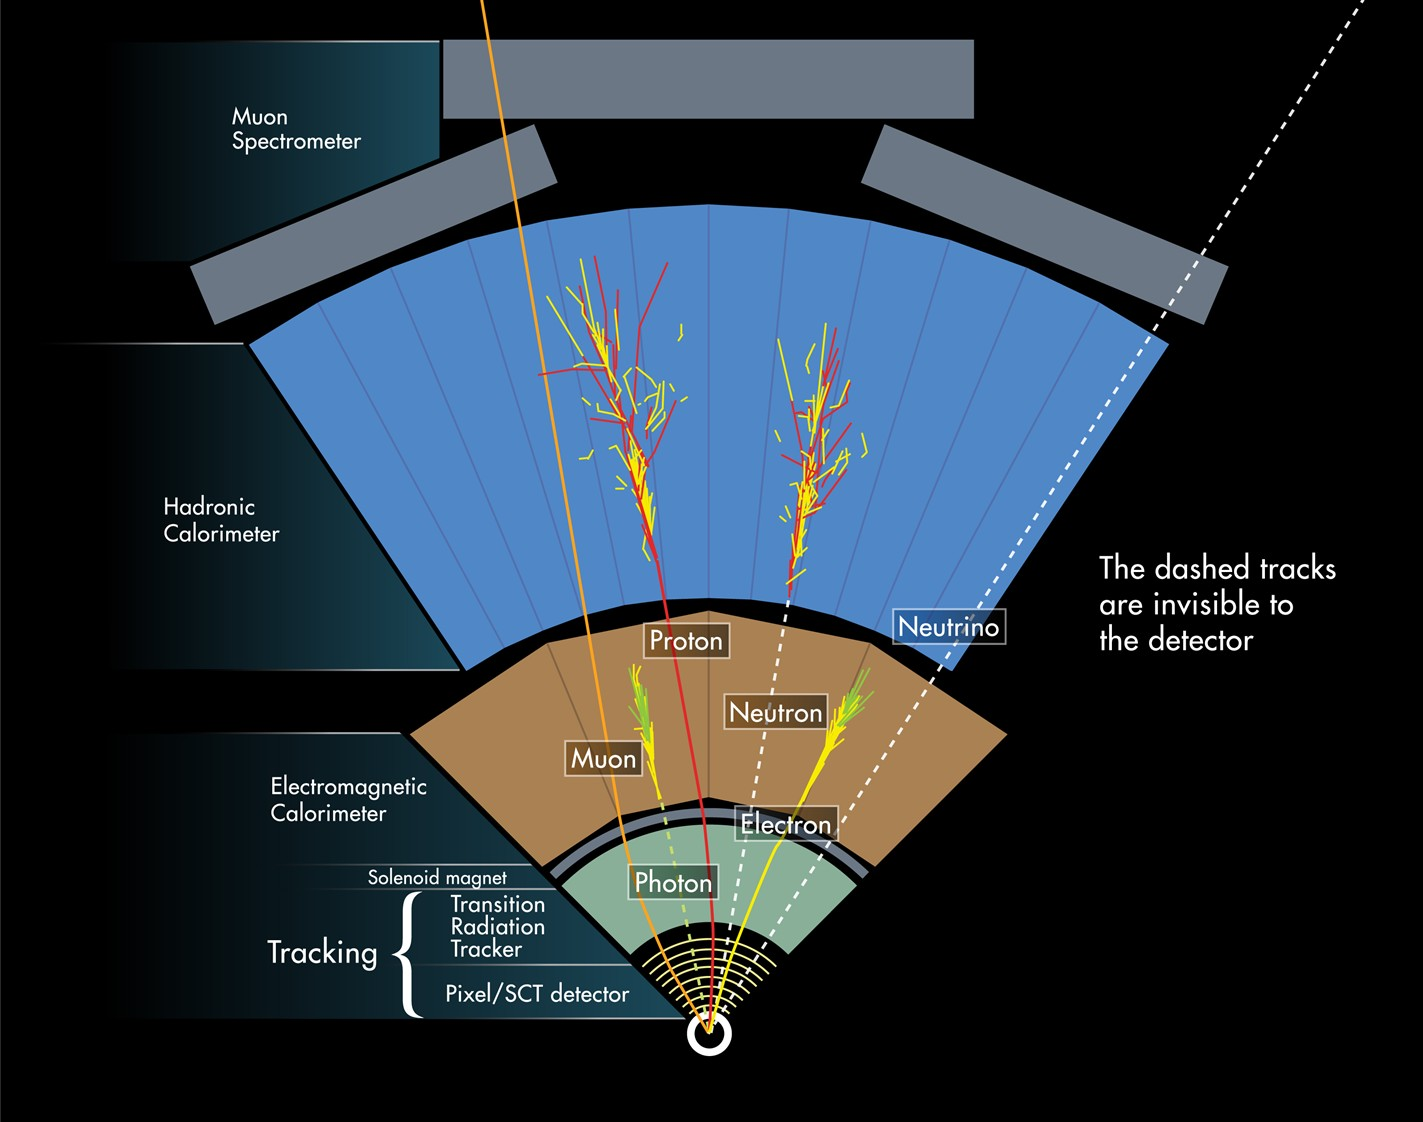
\includegraphics[width=0.8\textwidth]{figures/ATLAS-shower.jpeg}
		 }
\caption{Cross section of the ATLAS detector showing how particles interact with various detector components \cite{ShowerImage} \label{fig:ATLAS-shower}}
\end{figure}

\subsection{ATLAS Coordinate System} 
Of relevance for the following discussion, as well as for the analysis presented in Chapter \ref{chap:bbbb},
is the ATLAS coordinate system. ATLAS uses a right-handed coordinate system with its origin at the nominal 
interaction point (IP) in the center of the detector and the \(z\)-axis along the beam pipe.
The \(x\)-axis points from the IP to the centre of the LHC ring, and the \(y\)-axis points upwards.
Cylindrical coordinates \((r,\phi)\) are used in the transverse plane, \(\phi\) being the azimuthal angle 
around the \(z\)-axis. The pseudorapidity is defined in terms of the polar angle \(\theta\) as 
\(\eta = -\ln \tan(\theta/2)\). Angular distance is measured in units of 
\(\Delta R \equiv \sqrt{(\Delta\eta)^{2} + (\Delta\phi)^{2}}\). These coordinates are shown in Figure 
\todo{add coordinate figure}

\subsection{Inner Detector}

The inner-detector system (ID) is immersed in a \SI{2}{\tesla} axial magnetic field 
and provides charged-particle tracking in the range \(|\eta| < 2.5\).
The high-granularity silicon pixel detector covers the vertex region and typically provides four measurements per track, 
the first hit normally being in the insertable B-layer (IBL) installed before Run~2~\cite{ATLAS-TDR-19,PIX-2018-001}.
It is followed by the silicon microstrip tracker (SCT), which usually provides eight measurements per track.
These silicon detectors are complemented by the transition radiation tracker (TRT),
which enables radially extended track reconstruction up to \(|\eta| = 2.0\). 
The TRT also provides electron identification information 
based on the fraction of hits (typically 30 in total) above a higher energy-deposit threshold corresponding to transition radiation.

\subsection{Calorimeter}
The calorimeter system covers the pseudorapidity range \(|\eta| < 4.9\).
Within the region \(|\eta|< 3.2\), electromagnetic calorimetry is provided by barrel and 
endcap high-granularity lead/liquid-argon (LAr) calorimeters,
with an additional thin LAr presampler covering \(|\eta| < 1.8\)
to correct for energy loss in material upstream of the calorimeters.
Hadron calorimetry is provided by the steel/scintillator-tile calorimeter,
segmented into three barrel structures within \(|\eta| < 1.7\), and two copper/LAr hadron endcap calorimeters.
The solid angle coverage is completed with forward copper/LAr and tungsten/LAr calorimeter modules
optimised for electromagnetic and hadronic energy measurements respectively.

\subsection{Muon Spectrometer}
The muon spectrometer (MS) comprises separate trigger and
high-precision tracking chambers measuring the deflection of muons in a magnetic field generated by the superconducting air-core toroidal magnets.
The field integral of the toroids ranges between \num{2.0} and \SI{6.0}{\tesla\metre}
across most of the detector. 
A set of precision chambers covers the region \(|\eta| < 2.7\) with three layers of monitored drift tubes,
complemented by cathode-strip chambers in the forward region, where the background is highest.
The muon trigger system covers the range \(|\eta| < 2.4\) with resistive-plate chambers in the barrel, and thin-gap chambers in the endcap regions.

\subsection{Triggering}
Interesting events are selected by the first-level trigger system implemented in custom hardware,
followed by selections made by algorithms implemented in software in the high-level trigger~\cite{TRIG-2016-01}. 
The first-level trigger accepts events from the \SI{40}{\MHz} bunch crossings at a rate below \SI{100}{\kHz},
which the high-level trigger further reduces in order to record events to disk at about \SI{1}{\kHz}.

An extensive software suite~\cite{ATL-SOFT-PUB-2021-001} is used for real and simulated data reconstruction
and analysis, for operation and in the trigger and data acquisition systems of the experiment.
